% =====================================================================
% figB  — R/ggplot2 -> tikzDevice (parallel to ../figures-tex/figB_surrogate.tex)
% Canonical-JSON-only. Regenerate: Rscript figures-r/make_figures.R
% Provenance (JSON path :: field = plotted value), one line per series:
% SOURCE: results/C1_mechanism_sc_table.json :: groups[llama1b,L8].within_probe_rho_SC = 0.3899
% SOURCE: results/G2_gradsim_L8.json :: aggregate.gradsim_within_probe.resid.mean = 0.3899
% SOURCE: results/C1_mechanism_sc_table.json :: groups[llama1b,L10].within_probe_rho_SC = 0.5279
% SOURCE: results/G2_gradsim_L10.json :: aggregate.gradsim_within_probe.resid.mean = 0.5279
% SOURCE: results/C1_mechanism_sc_table.json :: groups[llama1b,L12].within_probe_rho_SC = 0.6278
% SOURCE: results/G2_gradsim_L12.json :: aggregate.gradsim_within_probe.resid.mean = 0.6277
% SOURCE: results/C1_mechanism_sc_table.json :: groups[llama1b,L14].within_probe_rho_SC = 0.4981
% SOURCE: results/G2_gradsim_L14.json :: aggregate.gradsim_within_probe.resid.mean = 0.4981
% =====================================================================
% !TEX encoding = UTF-8 Unicode
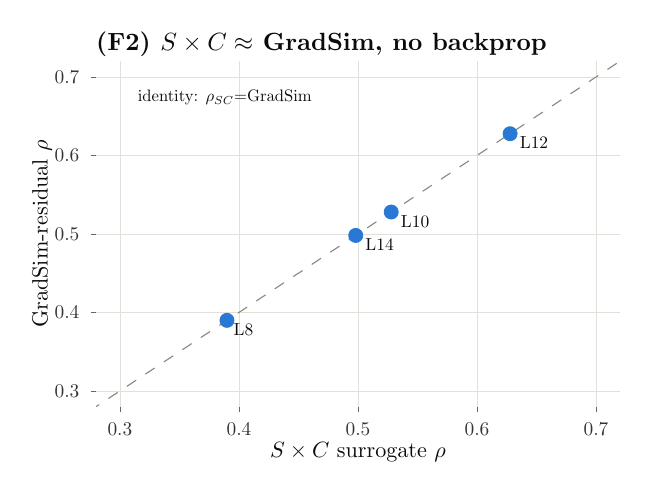
\begin{tikzpicture}[x=1pt,y=1pt]
\definecolor{fillColor}{RGB}{255,255,255}
\path[use as bounding box,fill=fillColor,fill opacity=0.00] (0,0) rectangle (218.98,158.99);
\begin{scope}
\path[clip] (  0.00,  0.00) rectangle (218.98,158.99);
\definecolor{fillColor}{RGB}{255,255,255}

\path[fill=fillColor] (  0.00,  0.00) rectangle (218.98,158.99);
\end{scope}
\begin{scope}
\path[clip] ( 24.74, 22.06) rectangle (213.98,146.84);
\definecolor{drawColor}{RGB}{225,224,217}

\path[draw=drawColor,line width= 0.3pt,line join=round] ( 24.74, 27.73) --
	(213.98, 27.73);

\path[draw=drawColor,line width= 0.3pt,line join=round] ( 24.74, 56.09) --
	(213.98, 56.09);

\path[draw=drawColor,line width= 0.3pt,line join=round] ( 24.74, 84.45) --
	(213.98, 84.45);

\path[draw=drawColor,line width= 0.3pt,line join=round] ( 24.74,112.81) --
	(213.98,112.81);

\path[draw=drawColor,line width= 0.3pt,line join=round] ( 24.74,141.17) --
	(213.98,141.17);

\path[draw=drawColor,line width= 0.3pt,line join=round] ( 33.34, 22.06) --
	( 33.34,146.84);

\path[draw=drawColor,line width= 0.3pt,line join=round] ( 76.35, 22.06) --
	( 76.35,146.84);

\path[draw=drawColor,line width= 0.3pt,line join=round] (119.36, 22.06) --
	(119.36,146.84);

\path[draw=drawColor,line width= 0.3pt,line join=round] (162.37, 22.06) --
	(162.37,146.84);

\path[draw=drawColor,line width= 0.3pt,line join=round] (205.38, 22.06) --
	(205.38,146.84);
\definecolor{drawColor}{RGB}{137,135,129}

\path[draw=drawColor,line width= 0.4pt,dash pattern=on 4pt off 4pt ,line join=round] (-164.50,-102.72) -- (403.22,271.63);
\definecolor{drawColor}{RGB}{42,120,214}
\definecolor{fillColor}{RGB}{42,120,214}

\path[draw=drawColor,line width= 0.3pt,line join=round,line cap=round,fill=fillColor] ( 72.01, 53.23) circle (  2.54);

\path[draw=drawColor,line width= 0.3pt,line join=round,line cap=round,fill=fillColor] (131.36, 92.37) circle (  2.54);

\path[draw=drawColor,line width= 0.3pt,line join=round,line cap=round,fill=fillColor] (174.32,120.67) circle (  2.54);

\path[draw=drawColor,line width= 0.3pt,line join=round,line cap=round,fill=fillColor] (118.54, 83.91) circle (  2.54);
\definecolor{drawColor}{RGB}{11,11,11}

\node[text=drawColor,anchor=base west,inner sep=0pt, outer sep=0pt, scale=  0.63] at ( 74.44, 47.73) {L8};

\node[text=drawColor,anchor=base west,inner sep=0pt, outer sep=0pt, scale=  0.63] at (134.89, 86.86) {L10};

\node[text=drawColor,anchor=base west,inner sep=0pt, outer sep=0pt, scale=  0.63] at (177.85,115.17) {L12};

\node[text=drawColor,anchor=base west,inner sep=0pt, outer sep=0pt, scale=  0.63] at (122.07, 78.41) {L14};

\node[text=drawColor,anchor=base west,inner sep=0pt, outer sep=0pt, scale=  0.60] at ( 39.79,132.14) {identity: $\rho_{SC}{=}$GradSim};
\end{scope}
\begin{scope}
\path[clip] (  0.00,  0.00) rectangle (218.98,158.99);
\definecolor{drawColor}{gray}{0.20}

\node[text=drawColor,anchor=base east,inner sep=0pt, outer sep=0pt, scale=  0.70] at ( 18.69, 25.46) {0.3};

\node[text=drawColor,anchor=base east,inner sep=0pt, outer sep=0pt, scale=  0.70] at ( 18.69, 53.82) {0.4};

\node[text=drawColor,anchor=base east,inner sep=0pt, outer sep=0pt, scale=  0.70] at ( 18.69, 82.17) {0.5};

\node[text=drawColor,anchor=base east,inner sep=0pt, outer sep=0pt, scale=  0.70] at ( 18.69,110.53) {0.6};

\node[text=drawColor,anchor=base east,inner sep=0pt, outer sep=0pt, scale=  0.70] at ( 18.69,138.89) {0.7};
\end{scope}
\begin{scope}
\path[clip] (  0.00,  0.00) rectangle (218.98,158.99);
\definecolor{drawColor}{gray}{0.40}

\path[draw=drawColor,line width= 0.3pt,line join=round] ( 22.74, 27.73) --
	( 24.74, 27.73);

\path[draw=drawColor,line width= 0.3pt,line join=round] ( 22.74, 56.09) --
	( 24.74, 56.09);

\path[draw=drawColor,line width= 0.3pt,line join=round] ( 22.74, 84.45) --
	( 24.74, 84.45);

\path[draw=drawColor,line width= 0.3pt,line join=round] ( 22.74,112.81) --
	( 24.74,112.81);

\path[draw=drawColor,line width= 0.3pt,line join=round] ( 22.74,141.17) --
	( 24.74,141.17);
\end{scope}
\begin{scope}
\path[clip] (  0.00,  0.00) rectangle (218.98,158.99);
\definecolor{drawColor}{gray}{0.40}

\path[draw=drawColor,line width= 0.3pt,line join=round] ( 33.34, 20.06) --
	( 33.34, 22.06);

\path[draw=drawColor,line width= 0.3pt,line join=round] ( 76.35, 20.06) --
	( 76.35, 22.06);

\path[draw=drawColor,line width= 0.3pt,line join=round] (119.36, 20.06) --
	(119.36, 22.06);

\path[draw=drawColor,line width= 0.3pt,line join=round] (162.37, 20.06) --
	(162.37, 22.06);

\path[draw=drawColor,line width= 0.3pt,line join=round] (205.38, 20.06) --
	(205.38, 22.06);
\end{scope}
\begin{scope}
\path[clip] (  0.00,  0.00) rectangle (218.98,158.99);
\definecolor{drawColor}{gray}{0.20}

\node[text=drawColor,anchor=base,inner sep=0pt, outer sep=0pt, scale=  0.70] at ( 33.34, 11.46) {0.3};

\node[text=drawColor,anchor=base,inner sep=0pt, outer sep=0pt, scale=  0.70] at ( 76.35, 11.46) {0.4};

\node[text=drawColor,anchor=base,inner sep=0pt, outer sep=0pt, scale=  0.70] at (119.36, 11.46) {0.5};

\node[text=drawColor,anchor=base,inner sep=0pt, outer sep=0pt, scale=  0.70] at (162.37, 11.46) {0.6};

\node[text=drawColor,anchor=base,inner sep=0pt, outer sep=0pt, scale=  0.70] at (205.38, 11.46) {0.7};
\end{scope}
\begin{scope}
\path[clip] (  0.00,  0.00) rectangle (218.98,158.99);
\definecolor{drawColor}{RGB}{11,11,11}

\node[text=drawColor,anchor=base,inner sep=0pt, outer sep=0pt, scale=  0.80] at (119.36,  3.73) {$S\times C$ surrogate $\rho$};
\end{scope}
\begin{scope}
\path[clip] (  0.00,  0.00) rectangle (218.98,158.99);
\definecolor{drawColor}{RGB}{11,11,11}

\node[text=drawColor,rotate= 90.00,anchor=base,inner sep=0pt, outer sep=0pt, scale=  0.80] at (  7.21, 84.45) {GradSim-residual $\rho$};
\end{scope}
\begin{scope}
\path[clip] (  0.00,  0.00) rectangle (218.98,158.99);
\definecolor{drawColor}{RGB}{11,11,11}

\node[text=drawColor,anchor=base west,inner sep=0pt, outer sep=0pt, scale=  0.90] at ( 24.74,150.79) {\bfseries (F2) $S\times C \approx$ GradSim, no backprop};
\end{scope}
\end{tikzpicture}
